\documentclass[12pt]{article}
\usepackage{pgfplots}
\usepackage{pgfplotstable}
\usepackage{movie15}
\usepackage{amsmath}
\usepackage{booktabs}
\usepackage{enumitem}
\usepackage{graphicx}
\usepackage{xcolor}
\usepackage{hyperref}
\usepackage{amssymb}
\usepackage{geometry}
\usepackage{physics}
\usepackage{listings}
\usepackage{lmodern}
\usepackage{float}
\usepackage{eso-pic}
\usepackage{lipsum}
\usepackage{comment}
\usepackage{balance}
\usepackage{tikz}
\usepackage{listings}
\usetikzlibrary{calc}
\usepackage{lscape}
\usepackage{color}

\usepackage{caption}
\usepackage{subcaption}

\definecolor{mygreen}{RGB}{28,172,0}
\definecolor{mylilas}{RGB}{170,55,241}
\newcommand{\n}{\newline}
\newcommand{\np}{\newpage}
\newcommand{\nn}{\newline \newline}
\newcommand{\timeofm}{$\mathcal{T}$}

\newcommand\tab[1][1cm]{\hspace*{#1}}
\floatplacement{figure}{H}
\newcommand{\Cross}{$\mathbin{\tikz [x=1.4ex,y=1.4ex,line width=.2ex, red] \draw (0,0) -- (1,1) (0,1) -- (1,0);}$}
\newcommand{\Checkmark}{$\color{black}\checkmark$}

\AddToShipoutPictureBG{
\begin{tikzpicture}[overlay,remember picture]
\draw[line width=4pt]
    ($ (current page.north west) + (1cm,-1cm) $)
    rectangle
    ($ (current page.south east) + (-1cm,1cm) $);
\draw[line width=.1pt]
    ($ (current page.north west) + (1.1cm,-1.1cm) $)
    rectangle
    ($ (current page.south east) + (-1.1cm,1.1cm) $);
\end{tikzpicture}
}

\geometry{left=2.5cm,right=2.5cm,top=2.5cm,bottom=2.5cm}
\lstset{ % Set the default style for code listings
	numbers=left, 
	numberstyle=\scriptsize, 
	numbersep=12pt,
	basicstyle=\scriptsize\ttfamily,
	keywordstyle=\color{blue},
	stringstyle=\color{red},
	commentstyle=\color{green!70!black},
	breaklines=true,
	frame=single, 
	language=MATLAB,
	tabsize=4,
	showstringspaces=false,
	captionpos=b
}

\title{
	
\includegraphics[width=0.5\textwidth]{UU_logo.jpg}\\[1em]
	High Performance Programming \\[1em]
	Assignment 3 \\[3em]
	Group 29
	\author{Kieran Barber, Panagiotis Papias}
}

\lstset{language=C,
    frame=tb,
    backgroundcolor=\color{white},   
    commentstyle=\color{dkgreen},
    keywordstyle=\color{blue},
    numbers=none,
    stringstyle=\color{carrotorange},
    basicstyle=\footnotesize,
    breakatwhitespace=false,         
    breaklines=true,                 
    captionpos=b,                    
    keepspaces=true,                 
    numbersep=5pt,                  
    showspaces=false,                
    showstringspaces=false,
    showtabs=false,                  
    tabsize=2,
    language=C
    
\begin{document}

\maketitle
\np
\tableofcontents
\np
\appendix



\section{The Problem}
For this assignment, we are going to implement a program that will calculate the evolution of N particles in a gravitational simulation, whereby we are given an initial set of particles. The simulation will be done in 2 spatial dimensions with an $x$ and $y$ coordinate. 
\\\\
To help describe the evolution of these particles, we will make use of Newton's law of gravitation in two dimensions, which states that the force exerted on particle $i$ by particle $j$ is given by
\\\\
    $$\boldsymbol{f}_{ij} = -\frac{Gm_{i}m_{j}}{\|\boldsymbol{r}_{ij}\|^{3}}\boldsymbol{r}_{ij}.$$
\\\\
where G is the gravitational constant, $m_{i}$ and $m_{j}$ are the masses of the particles, and $\boldsymbol{r}_{ij}$ is the distance vector given by $\boldsymbol{x}_{i} -\boldsymbol{x}_{j}$ with $x_{i}$ being the position of particle $i$. 
\\\\
We will make use of the following force equation (Plummer Sphere Force Equation) to describe the forces on the particles. The force on particle $i$ is given by
\\\\
    $$\boldsymbol{F}_{i} = -Gm_{i}\sum_{j = 0, j != i}^{N-1}\frac{m_{j}}{(\|\boldsymbol{r}_{ij}\| + \epsilon_{0})^{3}}\boldsymbol{r}_{ij}.$$
\\\\
where $\epsilon_{0}$ is a smoothing parameter and in the computations, we used the value $\epsilon = 10^{-3}$.
\\\\
To update the particle positions, we use the Euler Symplectic Time Integration method. The equations describing this are
\\\\
\begin{cases}
    $\boldsymbol{a}_{i}^{n} = \frac{\boldsymbol{F}_{i}^{n}}{m_{i}}$;
    \\
    $\boldsymbol{u}_{i}^{n+1} = \boldsymbol{u}_{i}^{n} + \Delta t\boldsymbol{a}_{i}^{n}$;
    \\
    $\boldsymbol{x}_{i}^{n+1} = \boldsymbol{x}_{i}^{n} + \Delta t\boldsymbol{u}_{i}^{n+1}$,
\end{cases}
\\\\
where $\Delta t$ is the time step size, $\boldsymbol{a}_{i}$ is the acceleration of particle $i$, $\boldsymbol{u}_{i}$ is the velocity and $\boldsymbol{x}_{i}$ is the position of particle $i$. In the computations, we used $\Delta t = 10^{-5}$. The value of G depends on N and is given by $G = 100/N$.
\newpage
\section{The Solution}
We began by writing our code in a file we named galsim.c. This is where all the functionality that we require is stored. We used code from graphics to be able to visualise the results of the simulation.
\\\\
Within the galsim.c file, we write our main program that will enable us to calculate the evolution of a system of N particles. This file begins with calling the relevant libraries we require. Below this, we take in the variables for the graphics, gravity and the smoothing constant epsilon. To improve runtime, we have set epsilon as a constant.
\\\\
Below this, we have our structs, one for the various vectors we will use and one for the particles attributes. The vector struct takes two doubles, one for $x$ and one for $y$. The particle struct takes two vectors for position and and velocity, and two doubles, one for mass and brightness. These have been ordered so that they are in the same order as the data that's read in from the gal-files.
\\\\
Below this, we introduced print functions that we would use for debugging. This includes print\_vector\_info, print\_particle\_info and print\_all\_particle\_info. After this, we include a function we then call in the main function to get computation times for each optimisation.
\\\\
We now look to the building of the force functions. Since the Plummer spheres force equation has smoothing involved, we looked to implement this. To do this, we built each component of the equation in separate functions. The first function to be built was $\boldsymbol{r}_{ij}$. We only computed this in one way. The next to compute was $r_{ij}^{3}$. This was implemented in two different ways.
\begin{center}
    Version 1
\end{center}
\begin{lstlisting}{language=C}
double norm3(vector_t v) {
    return pow((sqrt(pow((v.x), 2) + pow((v.y), 2)) + epsilon), 3);
}
\end{lstlisting}
\\\\
\begin{center}
    Version 2 - 4
\end{center}
\begin{lstlisting}{language=C}
double norm3(vector_t v) {
    double n3;

    n3 = sqrt(v.x*v.x + v.y*v.y) + epsilon; 
    n3 = n3 * n3 * n3; 
    return n3;
}
\end{lstlisting}
With the above versions of norm3, we then implemented them into two versions of a function to calculate the force on particle $i$ from particle $j$. To do this, we had to calculate in both the $x$ and $y$ directions. Initially, we chose to include all terms for both of these directions.
\begin{center}
    Version 1 - 2
\end{center}
\begin{lstlisting}{language=C}
vector_t force(particle_t pi, particle_t pj) {
    vector_t f;

    f.x = -(G * pi.mass * pj.mass * r_vector(pi.position, pj.position).x) 
            / norm3(r_vector(pi.position, pj.position));
    f.y = -(G * pi.mass * pj.mass * r_vector(pi.position, pj.position).y) 
            / norm3(r_vector(pi.position, pj.position));

    return f;
}
\end{lstlisting}
We decided then that we would calculate any repetitions in each equation just once, so that this may improve computation time. 
\begin{center}
    Version 3 - 4
\end{center}
\begin{lstlisting}{language=C}
vector_t force(particle_t pi, particle_t pj) {
    vector_t f;
    vector_t r;
    double a;

    r = r_vector(pi.position, pj.position);
    a = -(G * pi.mass * pj.mass) / norm3(r);

    f.x = a * r.x;
    f.y = a * r.y;

    return f;
}
\end{lstlisting}
Now that we have functions to compute the force applied to each particle, we can now loop through each particle, and compute the total force applied to each particle. 
\begin{center}
    Version 1 - 3
\end{center}
\begin{lstlisting}{language=C}
vector_t total_force(particle_t* p, int i, int N) {
    vector_t f = {0.0,0.0};
    
    for(int j = 0; j < N; j++) {
        if(i != j) {
            vector_t f_temp = force(p[j], p[i]);
            f.x += f_temp.x;
            f.y += f_temp.y;
        }
    }
    return f;
}
\end{lstlisting}
One final improvement we applied to this was to note that since we had the forces computed from particle $i$ to particle $j$, we also had the negative of this, so we then had the force applied from particle $j$ to particle $i$. 
\begin{center}
    Version 4
\end{center}
\begin{lstlisting}{language=C}
void compute_forces(vector_t* forces, particle_t* particles, int N) {

    for(int i = 0; i < N; i++) {
        forces[i].x = 0.0;
        forces[i].y = 0.0;
    }
    
    for(int i = 0; i < N; i++) {
        
        for(int j = i + 1; j < N; j++) {
                vector_t f = force(particles[j], particles[i]);
                forces[i].x += f.x;
                forces[i].y += f.y;

                forces[j].x -= f.x;
                forces[j].y -= f.y;
        }
        
    }
}
\end{lstlisting}
One final thing that we used to help us was to implement timings directly into the Makefile code so that when it came to computing wall timings at the end with different optimisations, we could do this directly from the Makefile. 
\section{CPU Configuration}
\begin{verbatim}
Architecture:        x86_64
CPU op-mode(s):      32-bit, 64-bit
Byte Order:          Little Endian
CPU(s):              8
On-line CPU(s) list: 0-7
Thread(s) per core:  2
Core(s) per socket:  4
Socket(s):           1
NUMA node(s):        1
Vendor ID:           GenuineIntel
CPU family:          6
Model:               142
Model name:          Intel(R) Core(TM) i5-8250U CPU @ 1.60GHz
Stepping:            10
CPU MHz:             700.041
CPU max MHz:         3400,0000
CPU min MHz:         400,0000
BogoMIPS:            3600.00
Virtualization:      VT-x
L1d cache:           32K
L1i cache:           32K
L2 cache:            256K
L3 cache:            6144K
NUMA node0 CPU(s):   0-7

(Ubuntu 7.4.0-1ubuntu1~18.04.1) 7.4.0

\end{verbatim}
\newpage
\section{Performance and Discussion}
\subsection{Timings}
\begin{center}
\begin{tabular}{|c|c|c|c|}
\hline
Version & -OO & -O3 & -Ofast\\
\hline
V1 & 199.702909 & 110.818015 & 3.372535\\
V2 & 94.216680 & 4.225227 & 4.065753\\
V3 & 45.380386 & 3.521552 & 3.271567\\
V4 & 24.352817 & 2.538566 & 2.454337\\
\hline
\end{tabular}
\end{center}
Given the optimisations described through code changes in the previous section, we have above, our timings for various optimisation flags. 
\\\\
Starting with Version 1, we can see that setting no optimisation flags to the code leaves us computing for a significant amount of time. this is almost halved by taking the -O3 flag. The -Ofast flag takes a significantly shorter amount of time to compute this system. A potential reason we can see here is that it sees the use of the pow function and realises it just simply needs to compute $x*x$ rather than $x^2$ for instance. 
\\\\
The second version of the code that we produced moved from calculating norm3 in the version we described above. This gave significant increases in time performance for the -O0 and -O3 flags, however, it actually increased computation time for the -Ofast flag. We have not understood why this is the case. 
\\\\
For Version 3, we altered the way in which we computed the force for each particle. Instead of calling functions for both the x and y directions, we decided to take out the elements of each equation that are the same and compute them before we computed the force in each of the $x$ and $y$ directions, thus meant that we were doing half of the original calculations. Again, this gave significant improvements in performance for -O0. Proportionately, it gave big performance improvements for -O3 and -Ofast. 
\\\\
The final Version took into account that we could compute the forces in half the time. This is achieved since once we know the force applied to particle $i$ from particle $j$, we know that the force applied to particle $j$ from particle $i$ is just the negative. This gave significant performance improvements with each flag. 
\begin{figure}[htb]
\begin{center}
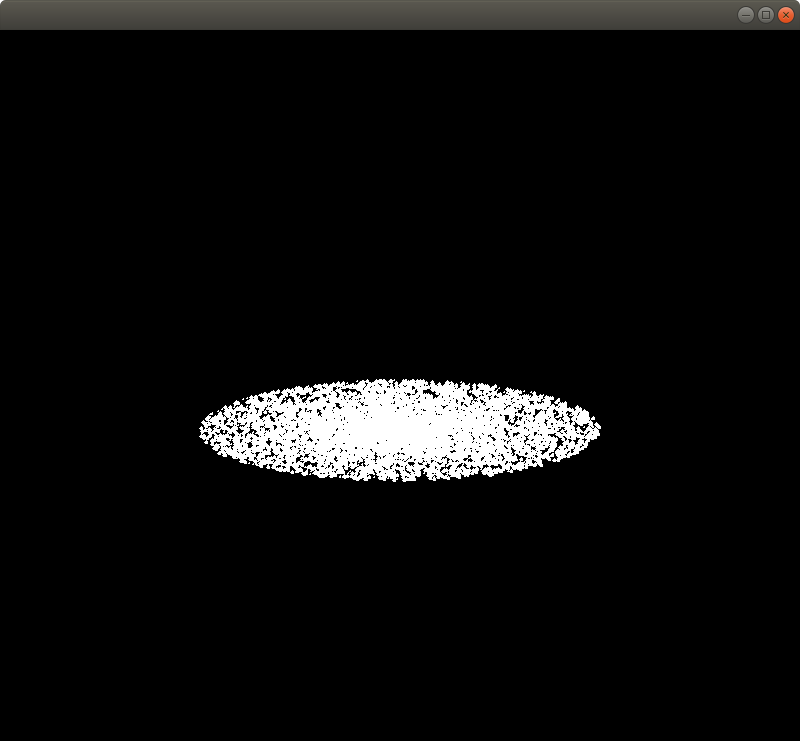
\includegraphics[width=6cm]{space.jpg}
\caption{A simulation of a galaxy}
\end{center}
\end{figure}
\newpage
\subsection{Complexity}
Finally, below we have a plot outlining the computation times measured against $O(N^{2})$.
\begin{figure}[htb]
\begin{center}
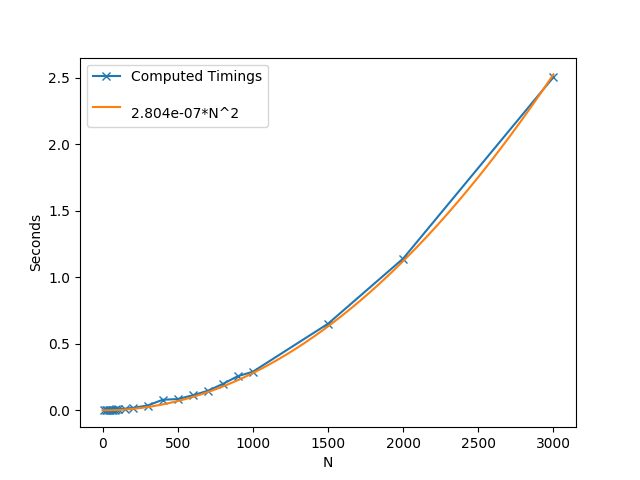
\includegraphics[width=14cm]{time_complexity.png}
\caption{Time Complexity Plot}
\end{center}
\end{figure}


\end{document}